


Байесовы сети применяются в причинно-следственном анализе.

Итоговая модель представляет собой статистическую модель явления, которую можно использовать для
управления и анализа системой. 
Описанный подход называется \textit{вариационным причиннно-следственным выводом}.

В теории причинно-следственного анализа введенную величину
свидетельство. (\texit{англ.} Evidence).

Максимизация свидетельства
позволяет выбирать модели согласно принципу бритву Оккама, исключая
параметры не вносящие существенного смысла для модели. Для расчета свидетельства необходимо выполнить маргинализацию по параметрам
модели $\int P(X, \theta) d\theta$. В общем случае задача принадлежит 
NP-классу сложности, рассчитывается за время, экспоненциально зависящее
от числа параметров. 

\texit{Определение} События $A$ и $B$ cчитаются независимыми в условиях:
\begin{equation}
    P(A \cup B) = P(A) \times P(B)
\end{equation}

На практике в системах подлинная независимость случайных величин $x$ и $y$
$x \perp y$ встречается не всегда. Чаще достижима условная независимость, наблюдаемая при
фиксации третьего фактора $z$.

\texit{Определение} События $A$ и $B$ cчитаются условно независимыми 
для заданного события $C$ в условиях:
\begin{equation}
    P(A \cup B |C) = P(A|C) \times P(B|C)
\end{equation}

\begin{figure}[h]
    \centering
    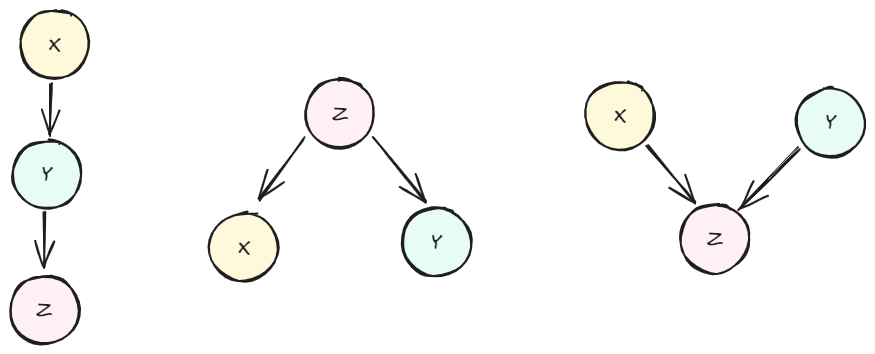
\includegraphics[width=0.5\textwidth]{assets/math/discrete/bayes_net.excalidraw.png}
    \caption{Посредник(\textit{англ.} mediator), общий предок(\textit{англ.} cofounder), 
 общий родственник (\textit{англ.} collider) }
    \label{discr_vs_gen}
\end{figure}

Виды вариационного вывода можно разделить на три ключевых направлениях: \begin{itemize}
    \item прогнозирование
    \item обратный - объяснение причины на основании
\end{itemize}

Вывод выполняется путем маргинализации распределения по 



Многокомпонетный осложняется неоднозначной трактовкой исхода. 
Для анализа сложных систем предпочтителен однофакторный анализ, выполняющий
для его выполнения необходимо перекрыть потоки зависимостей (\textit{англ.} dependency flow) от
прочих переменных.

\texit{Определение} \textbf{Интервенцией} называется изменение 

\begin{figure}[h]
    \centering
    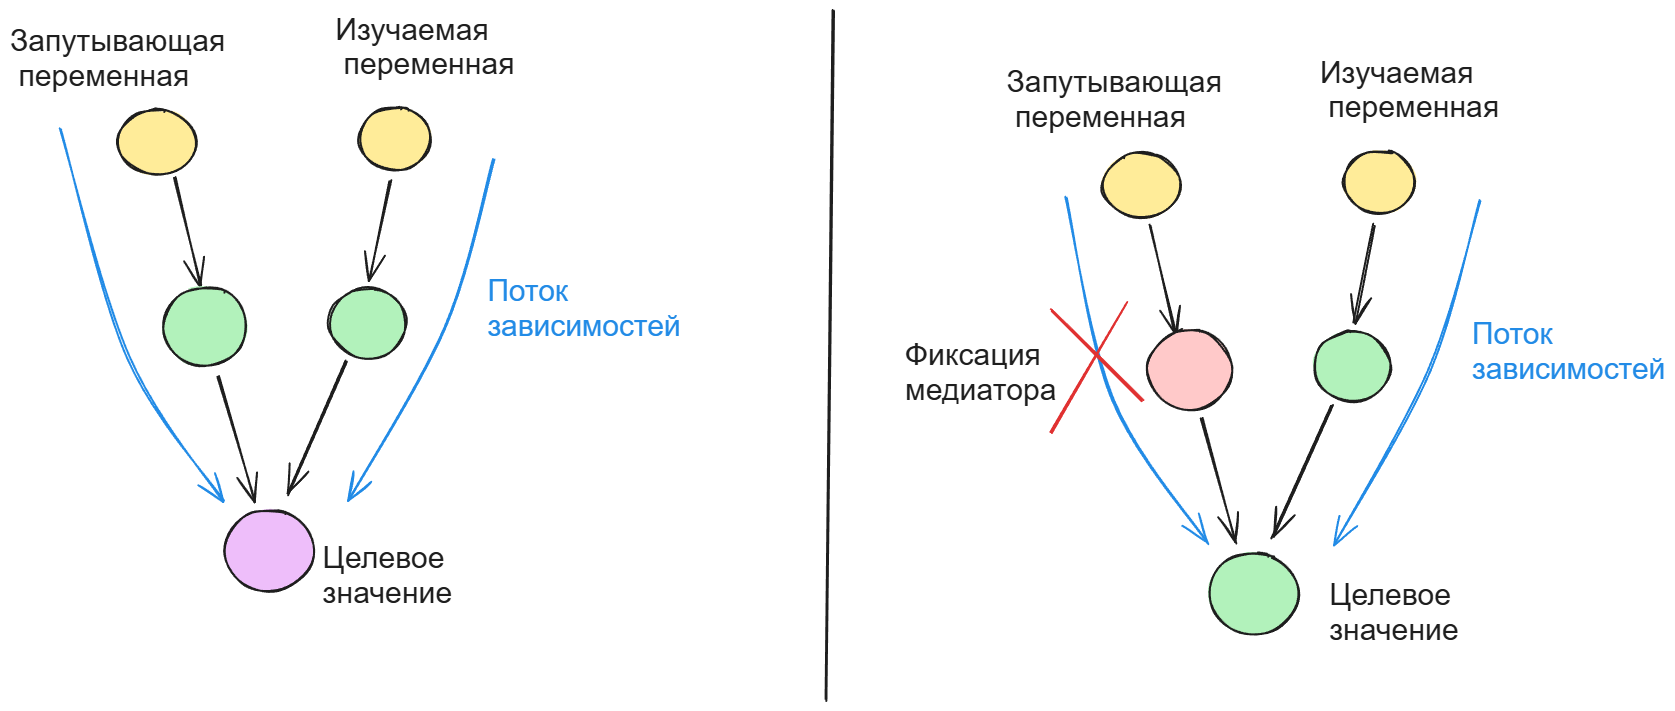
\includegraphics[width=0.5\textwidth]{assets/math/discrete/dep_flow.excalidraw.png}
    \caption{Интервенция}
    \label{discr_vs_gen}
\end{figure}

\texit{Определение} События $A$ и $B$ cчитаются независимыми в условиях:
\begin{equation}
    P(A \cup B) = P(A) \times P(B)
\end{equation}

\begin{figure}[h]
    \centering
    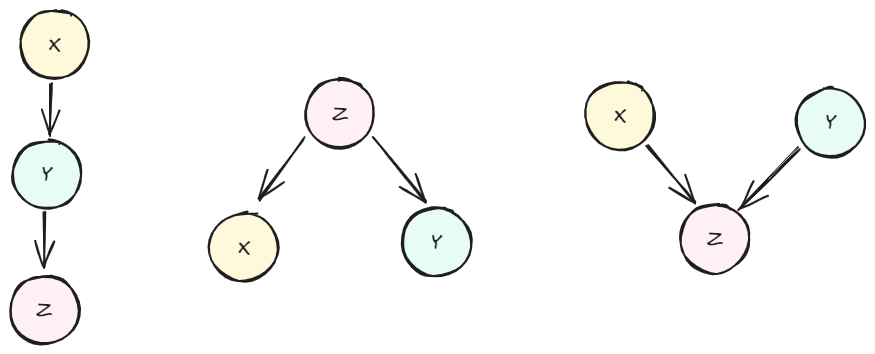
\includegraphics[width=0.5\textwidth]{assets/math/discrete/bayes_net.excalidraw.png}
    \caption{Посредник(\textit{англ.} mediator), общий предок(\textit{англ.} cofounder), 
 общий родственник \textit{англ.} collider) }
    \label{discr_vs_gen}
\end{figure}




Условная независимость позволяет 
$x \perp y$ встречается не всегда.


